\chapter{Paquímetro}

%====================
\section{Objetivo}
\begin{itemize}
\item Conhecer o \emph{paquímetro} como instrumento de medida.
\item Realizar medidas simples de objetos com geometria regulares.
\item Realizar medidas utilizando profundidade, diâmetros internos e externos.
\end{itemize}





%===================
\section{Material Utilizado}
%Aqui vamos identificar todos os materiais e equipamento utilizados no experimento.

\begin{itemize}
	\item Paquímetros de diferentes precisões ($0,05$ e $0,02\;mm$);
	\item Blocos metálicos de geometrias regulares;
\end{itemize}%





%==========
\section{Fundamentos Teóricos}

A Física é chamada uma ciência exata. Entretanto, nas práticas de laboratório, em geral, os instrumentos não fornecem medidas exatas.
Quando medimos o comprimento de uma peça metálica com uma régua de plástico, em um dia frio ($\approx 5 {^\circ C}$) encontramos um certo valor.
Agora, se medimos o mesmo comprimento da mesma peça metálica em um dia quente ($\approx 40 {^\circ C}$) poderemos observar uma pequena diferença da medida anterior.
É importante e necessário fazer um curso de Física Experimental e tentar descobrir e estimar os erros de medições existentes.

O Paquímetro é um instrumento de alta precisão usado em oficinas e laboratórios, projetado para a tomada de medidas lineares de comprimento nas mais diversas modalidades:
\begin{itemize}
\item Dimensões lineares internas e externas;
\item Espessuras;
\item Rebaixos;
\item Profundidades de peças, etc.
\end{itemize}

O paquímetro, mostrado na \autoref{fig:paquimetro005}, é composto de uma parte fixa chamada haste, e por uma parte móvel chamada cursor. No cursor está gravada a escala auxiliar denominada \emph{nônio} ou \emph{vernier}.

\begin{figure}[!htb]
\centering
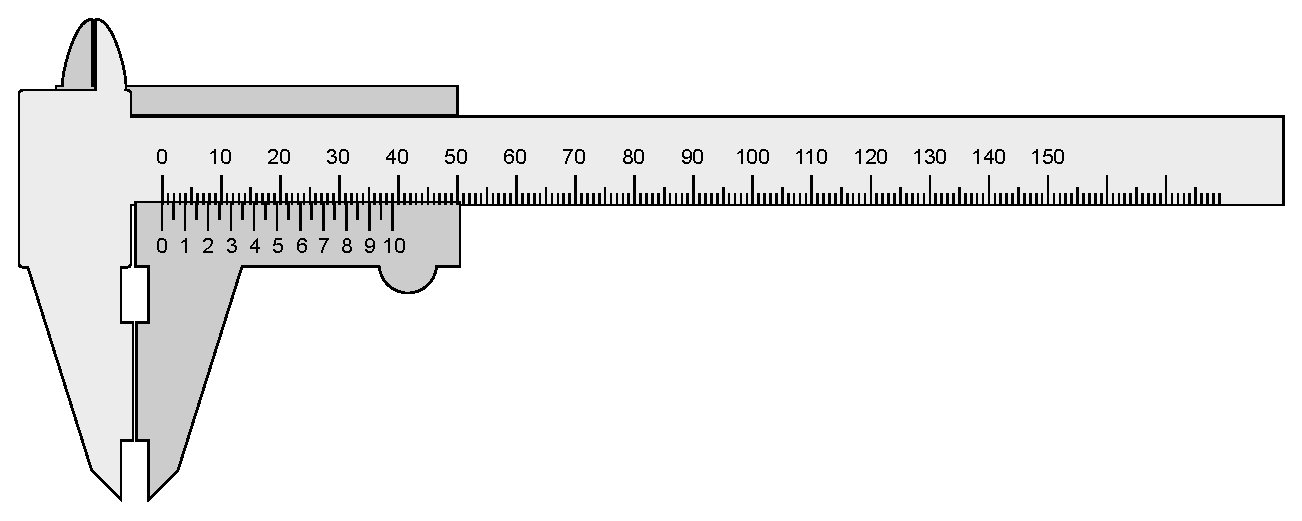
\includegraphics[scale=0.7]{figs/paquimetro005.eps}
\caption{Paquímetro analógico de resolução $0,05\;mm$.}
\label{fig:paquimetro005}
\end{figure}

Para determinarmos a precisão de um paquímetro devemos observar duas coisas: o menor intervalo da escala fixa, e a quantidade de intervalos existentes na nônio\footnote{Não confundir a quantidade de intervalos com a numeração apresentada.}.
No exemplo da \autoref{fig:paquimetro005} observamos que a escala fixa possui o menor intervalo de $1\;mm$, e que a escala móvel possui $20$ intervalos. Logo este paquímetro possui precisão de $1\;mm / 20 = 0,05\;mm$!

A leitura de um paquímetro é muito semelhante à leitura de uma régua convencional. A única diferença é que no paquímetro precisamos levar em conta a leitura do nônio. Para entendermos a fazer tal leitura, vamos utilizar o exemplo da \autoref{fig:paquimetro005_zoom}.


\begin{figure}[!htb]
\centering

\includegraphics[scale=1.5]{figs/paquimetro005_zoom1_test.eps}
\caption{Leitura da escala fixa do paquímetro, tomando como referência o zero da escala móvel. Leitura de $16\;mm$.}
\label{fig:paquimetro005_zoom}
\end{figure}





%===================================================
\section{Procedimento Experimental}
%Aqui vamos guiar o leitor através do experimento para que o mesmo possa realizá-lo sem muitos problemas.

\begin{enumerate}[leftmargin=*]

\item Determine as dimensões e o volume do paralelepípedo de metal e registre os valores na \autoref{tab:paralelepipedo}. Repita 3 vezes cada medida, escrevendo corretamente seus algarismos significativos, assim como o erro absoluto.
%\anotacoes{0.6cm}

%Tabela gerado no Lyx.
\begin{table}[H]
\centering{}%
\caption{Medidas das dimensões do paralelepípedo em milímetro.}
\label{tab:paralelepipedo}
\renewcommand*\arraystretch{1.25} %Altura das linhas
\begin{tabular}{|c|c|c|c|c|}
\hline 
\multirow{5}{*}{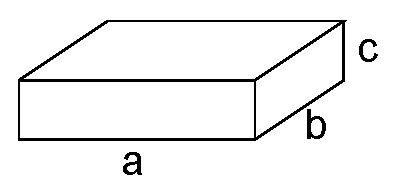
\includegraphics[scale=0.6]{figs/paralelepipedo.eps}} & Medidas & a & b & c\tabularnewline
\cline{2-5} 
 & 1 & $\hspace{1.5cm}$ & $\hspace{1.5cm}$  & $\hspace{1.5cm}$ \tabularnewline
\cline{2-5} 
 & 2 &  &  & \tabularnewline
\cline{2-5} 
 & 3 &  &  & \tabularnewline
\cline{2-5} 
 & Média &  &  & \tabularnewline
\hline 
\end{tabular}
\end{table}



\begin{table}[H]
\centering{}%
\caption{Medidas das dimensões do cilindro em milímetro.}
\label{tab:cilindro}
\renewcommand*\arraystretch{1.25} %Altura das linhas
\begin{tabular}{|c|c|c|c|}
\hline 
\multirow{5}{*}{
\includegraphics[scale=0.9]{figs/cilindro.eps}} & Medidas & D & h \tabularnewline
\cline{2-4} 
 & 1 & $\hspace{1.5cm}$ & $\hspace{1.5cm}$  \tabularnewline
\cline{2-4} 
 & 2 &  & \tabularnewline
\cline{2-4} 
 & 3 &  & \tabularnewline
\cline{2-4} 
 & Média &  & \tabularnewline
\hline 
\end{tabular}
\end{table}



\begin{table}[H]
\centering{}%
\caption{Medidas das dimensões da esfera em milímetro.}
\label{fig:esfera}
\renewcommand*\arraystretch{1.25} %Altura das linhas
\begin{tabular}{|c|c|c|}
\hline 
\multirow{5}{*}{
\includegraphics[scale=0.9]{figs/esfera.eps}} & Medidas & D \tabularnewline
\cline{2-3} 
 & 1 & $\hspace{1.5cm}$  \tabularnewline
\cline{2-3} 
 & 2 & \tabularnewline
\cline{2-3} 
 & 3 & \tabularnewline
\cline{2-3} 
 & Média & \tabularnewline
\hline 
\end{tabular}
\end{table}




\end{enumerate}



%==========

%%Precisa do pacote: \usepackage{pifont}
%\noindent\dotfill
%\ding{33}\dotfill
%\raisebox{-0.25\baselineskip}{\ding{34}}\dotfill
%\raisebox{-0.50\baselineskip}{\ding{35}}\dotfill

\newpage
\section{Questionário}
%Aqui vamos inserir perguntas/questionamentos sobre a prática para que o leitor/aluno possa melhorar o aprendizado.


\begin{enumerate}[leftmargin=*]

\item Pode-se concluir a respeito do experimento que os períodos independem da massa? Justifique.
\anotacoes{2cm}

\item O que se pode concluir a respeito dos períodos quando a amplitude de oscilação variou de $10^{\circ}$ para $15^{\circ}$? Justifique.
\anotacoes{2cm}

\item Determine o valor da aceleração da gravidade local à partir do gráfico $T^2 \times L$.
\anotacoes{2cm}

\item Calcule o valor de $T$ para um pêndulo com $L=140\;cm$ e $g=9,8\;m/s^2$ usando a \autoref{eq:periodo}. Compare com o valor experimental.
\anotacoes{2cm}

\item Qual o peso de um aluno de massa $60,0\;kg$ no local onde foi realizada a experiência?
\anotacoes{2cm}

\end{enumerate}

%\cleardoublepage
%\includepdf[pages={1}]{figs/Graph_paper_mm_A4_black.pdf}


